\documentclass[12pt]{elsarticle}

\usepackage{lineno,hyperref,notoccite,etoolbox}
\makeatletter
\def\ps@pprintTitle{%
	\let\@oddhead\@empty
	\let\@evenhead\@empty
	\def\@oddfoot{\centerline{\thepage}}%
	\let\@evenfoot\@oddfoot}
\makeatother
\usepackage{setspace}
\singlespacing
\usepackage{mathptmx}
\usepackage{float,wrapfig}
\usepackage[margin=1in]{geometry}
\usepackage{booktabs}
\usepackage{cancel}
\usepackage[fleqn]{amsmath}
\usepackage{amssymb}
\allowdisplaybreaks
\newcommand{\bnumbers}{\begin{enumerate}}
	\newcommand{\enumbers}{\end{enumerate}}
\newcommand{\vs}{\vspace{2mm}}
\newcommand{\beq}{\begin{equation*}}
\newcommand{\eeq}{\end{equation*}}
\newcommand{\rr}[1]{\mbox{#1}}
\newcommand{\longequals}{{=\joinrel=}}
\newcommand{\squared}{$^{2}$}
\newcommand{\subtwo}{$_{2}$}
%tables
\setlength{\arrayrulewidth}{0.5mm}
\setlength{\tabcolsep}{5pt}
\renewcommand{\arraystretch}{1.75}
\newcommand{\fullline}{\noindent\rule{14cm}{0.4pt} \vspace{4mm}}
\usepackage{subfigure}



\begin{document}
\begin{flushright}
	Ember Sikorski\par
	Homework 2\par
	ECE 624\par 
	5 October 2018
\end{flushright}


\begin{enumerate}
%1	
\item Explain why electronic doping by introduction of suitable donor/acceptor levels in an amorphous material is difficult. \par \vs
Electronic doping is difficult is amorphous materials due to the high concentration of instrinsic states in the gap \cite{Tauc1976}. When dopants are added, the concentration of introduced states is low compared to the intrinsic states, making it difficult to move the Fermi level. Additionally, with their low coordination number and flexibility, amorphous materials can undergo relaxation when dopants are added \cite{Kim2015}. This traps the added charge carriers instead of producing a system with more free carriers. This can be modeled with VAPs, which can use the added carriers to change the charge of their dangling bond \cite{Fritzsche2007}. To introduce a large enough number of states to move the Fermi level, the  number of dopants must be at least double the number of VAP defects \cite{Fritzsche2007}.

\fullline
%2
\item Explain why the doping discussed in problem (1) might not improve carrier mobility. \par \vs
Doping introduces charged defects,D$^{+}$ and D$^{-}$, and though these defects are only capable of trapping either electrons \emph{or} holes respectively,  they are much more effective trap sites than D$^{0}$ \cite{Street1983}. Street et al. found D$^{+}$ centers were 5 times more effective than D$^{0}$ centers at trapping eletrons and D$^{-}$ centers were 2-4 times more effective at trapping holes than D$^{0}$ centers. Similarly, Kazakova and Tsendin \cite{Kazakova1999} found that when the number of dopants is 2 to 3 times the number of defect centers, hole mobility decreases as dopant concentration increases.
\fullline
%3
\item Would you expect to see blocking contacts in a metal-amorphous semiconductor contact? Explain your answer. \par \vs 
I would expect to see blocking contacts because of the high concentration of trap states in an a-semiconductor. Until these traps are filled, one would observe an ohmic contact at low voltages ~10V \cite{Singh2006}. However, once the states are filled, a-semiconductors exhibit space charge limited conduction (SCLC) \cite{Singh2006,Kushwaha2006,MajeedKhan2003} where carriers from the metal can only enter states in the semiconductor as carriers move from those states. High voltages (~10$^{4}$V/cm$^2$) are then needed to overcome SCLC and reach superohmic behavior\cite{Singh2006,Kushwaha2006}.

\fullline
%4
\item Describe the structural order giving rise to extended (delocalized) states and localized states in an amorphous semiconductor. \par \vs 

Localized states can come from defects like VAPs while extended states consist of the more stable ``happy" charge carriers. Drabold et al. \cite{Drabold2000} describe this quantum mechanically by considering ``severe distortions'' or the bonds that deviate the greatest from a tetrahedral structure in the case of a-Si. As larger distortions are less likely to occur, there is less degeneracy and especially so if those disorted clusters are isolated. As distortions become less severe, they are more likely to occur and lead to mixing of states. This was seen by mapping energy resolved states (e.g. near the Fermi level, at the valence band tail, etc.) to the structure. Near the Fermi level the authors found charge localized to a small cluster exhibiting very high distortion. As they shifted the energy window towards the valence band the cluster became larger. Finally, when examining the deep valence band states the charge mapped to several small clusters. In short, localized states originate in regions with the greatest structural disorder, while extended states come from regions of ``ideal'' structure, in this case tetrahedral.
\begin{figure}
	\hfill
	\subfigure[]{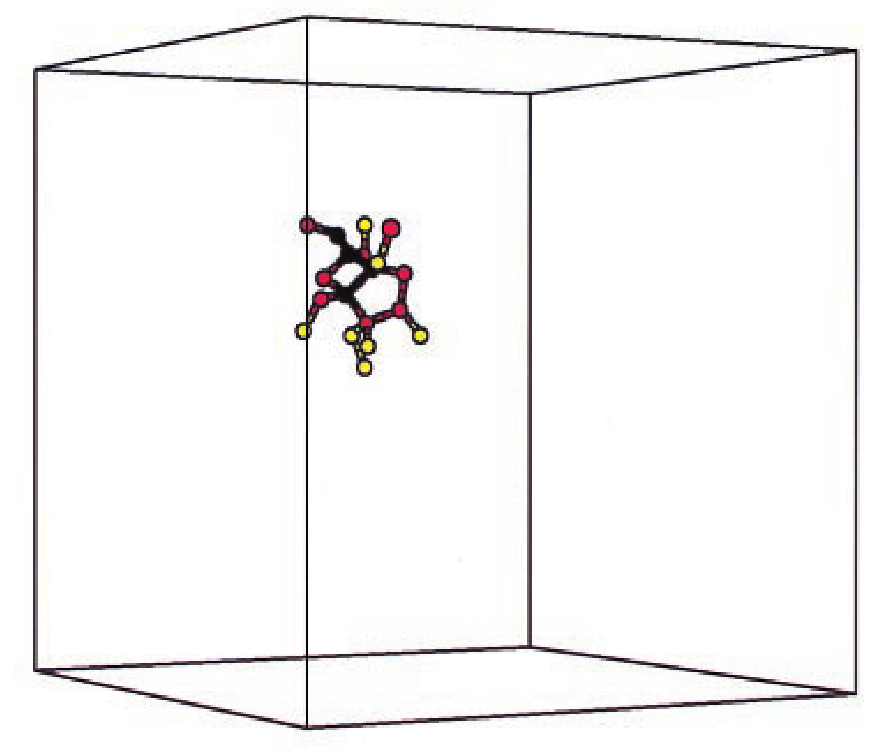
\includegraphics[width=5cm]{loc}}
	\hfill
	\subfigure[]{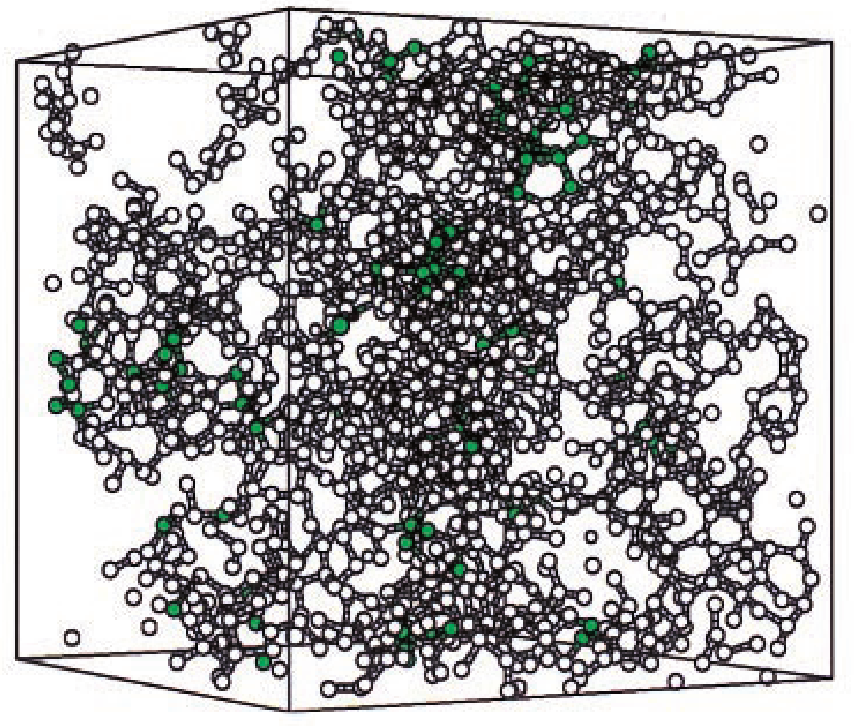
\includegraphics[width=5cm]{deloc}}
	\hfill
	\caption{Selected results from Drabold et al. \cite{Drabold2000} of structure contributing to (a) midgap states and (b) extended states. Color represents charged regions.}
\end{figure}

\fullline
%5
\item Provide definitions/explanations of the following:
\begin{itemize}
	\item Hubbard correlation energy
	\item Localization length
	\item Anderson transition \par \vs
	The Anderson transition describes the change from localized states in the band gap to extended or delocalized states. \cite{Drabold2000}
	\item Localized ``in the Anderson sense"
\end{itemize}
\fullline
%6
\item \begin{enumerate}
	\item What is the difference between variable range hopping and nearest neighbor hopping?
	\item In which type of conduction will tunneling occur?
\end{enumerate}

\end{enumerate}

\section*{References}
\bibliography{homework2}
\bibliographystyle{elsarticle-num}


\end{document}  